\documentclass{article}

\usepackage[english]{babel}     %testi autogenerati italiano
\usepackage{graphicx}           %per importare immagini
\usepackage{geometry}           %per gestire margini e spostamenti
\usepackage[raggedright]{titlesec}
\geometry {
    top=20mm,
    bmargin=20mm,
}
\usepackage{array}              %per colonne di width fissata
\usepackage{subcaption}         %tabelle divise
\usepackage{hyperref}           %links
\hypersetup{
    colorlinks=true,
    linkcolor=black,
    urlcolor=blue
}
%\usepackage[bottom]{footmisc}   %footnotes fissate a piè pagina
\usepackage{booktabs}           %per tabitem in tabular
\newcommand{\tabitem}{~~\llap{\textbullet}~~}
\renewcommand*{\thefootnote}{[\arabic{footnote}]}


\usepackage{tikz-er2}
\usepackage{geometry}
%\usepackage{lscape}
\usetikzlibrary{shadows,positioning}

\tikzset{every entity/.style = {top color=white,bottom color=blue!30,draw=blue!50!black!100,drop shadow},
every attribute/.style = {top color=white, bottom color=yellow!20,draw=yellow, drop shadow},
every relationship/.style = {top color=white, bottom color=red!20,draw=red!50!black!100, drop shadow},
every edge/.style={link},
every isa/.style = {top color=white, bottom color=green!20,draw=green!50!black!100, drop shadow}
}





\usepackage{caption}

\usepackage[section]{minted} % For code blocks
\newenvironment{code}{\captionsetup{type=listing}}{}
\usepackage[many]{tcolorbox}
\tcbuselibrary{minted}

\newtcbinputlisting{\mycode}[2]{%
  listing engine=minted,
  minted language={#1},
  listing file={#2},
  minted options={
    autogobble=true,
    baselinestretch=1.2,
    fontsize=\footnotesize,
    breaklines=true,
    encoding=utf8
    },
  listing only,
  breakable,
  enhanced jigsaw,
  colframe=black,
  sharp corners,
  boxrule=1pt,
  colback=lightgray!10,
  width=\linewidth
}

%remove red square
\usepackage{etoolbox,xpatch}
\makeatletter
\AtBeginEnvironment{minted}{\dontdofcolorbox}
\def\dontdofcolorbox{\renewcommand\fcolorbox[4][]{##4}}
\xpatchcmd{\inputminted}{\minted@fvset}{\minted@fvset\dontdofcolorbox}{}{}
\xpatchcmd{\mintinline}{\minted@fvset}{\minted@fvset\dontdofcolorbox}{}{} % see https://tex.stackexchange.com/a/401250/
\makeatother


% The following code is only to create the query files
\usepackage{filecontents}
%query1
\begin{filecontents*}{query1.v}
MATCH (x:Infected) 
RETURN x.p06_infectionDate, count(*)
\end{filecontents*}
%query2
\begin{filecontents*}{query2.v}
MATCH (x:Infected)-[r:VISITS]-(p:Place)
WHERE duration.inDays(x.p06_infectionDate, r.date).days <= 2
WITH count(r) as c, p.p02_type as type
RETURN type,c
\end{filecontents*}
%query3
\begin{filecontents*}{query3_1.v}
MATCH (a:Infected)-[v1:VISITS]-(p:Place)-[v2:VISITS]-(b:Person)
WITH duration.inDays(v1.date, a.p06_infectionDate).days AS DAYS_INTERVAL, b, v2, p
WHERE
NOT b:Infected AND
 v1.date = v2.date AND
 DAYS_INTERVAL > 0 AND
 DAYS_INTERVAL < $exposure_interval
RETURN b.p01_name AS Name, b.p02_surname AS Surname, v2.date AS DateOfContact,
p.p01_name AS PlaceOfContact
\end{filecontents*}

%query4
\begin{filecontents*}{query3_2.v}
MATCH (a:Infected)-[r:MEETS]-(b:Person)
WITH duration.inDays(r.date, a.p06_infectionDate).days AS DAYS_INTERVAL, b, r
WHERE
NOT b:Infected AND
DAYS_INTERVAL > 0 AND
DAYS_INTERVAL < $exposure_interval
RETURN b.p01_name AS Name, b.p02_surname AS Surname, r.date AS DateOfContact, r.place AS
PlaceOfContact
\end{filecontents*}

%query5
\begin{filecontents*}{query4.v}
CALL {
  MATCH (p:Infected)-[d2:VISITS]->(place:Place)<-[d1:VISITS]-(unfortunateSoul:Person)
  WHERE p.p06_infectionDate <= d1.date AND d1.date = d2.date 
        AND NOT unfortunateSoul:Infected
  WITH count(unfortunateSoul) AS total1
  RETURN total1
}
CALL {
  MATCH (p2:Infected)-[d1:MEETS]->(unfortunateSoul:Person)
  WHERE p2.p06_infectionDate <= d1.date AND NOT unfortunateSoul:Infected
  WITH count(unfortunateSoul) AS total2
  RETURN total2
}
CAll{
MATCH (p3:Infected)-[d2:FAMILY_CONTACT]->(unfortunateSoul:Person)
WHERE NOT unfortunateSoul:Infected
WITH count(unfortunateSoul) AS total3
RETURN total3}
CALL{
MATCH (N:Infected)
RETURN count(N) AS totalInfected}
RETURN total1 * 1.0 / totalInfected, total2 * 1.0 / totalInfected, total3 * 1.0 / totalInfected
\end{filecontents*}
\begin{filecontents*}{query5.v}
MATCH (x:Infected) RETURN x.p04_vaccine, COUNT(*)
\end{filecontents*}
\begin{filecontents*}{query6.v}
MATCH (x) RETURN x.p04_vaccine, COUNT(*)
\end{filecontents*}


%command1
\begin{filecontents*}{command1.v}
MATCH (n : Person{p01_name:$name, p02_surname:$surname}), (t:$test_type)
CREATE (n)-[r:TEST{date:$date,result:$test_result}]->(t)
FOREACH (p IN CASE WHEN r.result = true THEN[1] ELSE[] END | SET n.p06_infectionDate = r.date, n:Infected)
FOREACH (p IN CASE WHEN (r.result = false AND (NOT HAS(n.p06_infectionDate) OR n.p06_infectionDate < r.date)) THEN[1] ELSE[] END |  REMOVE n.p06_infectionDate, n:Infected);
\end{filecontents*}

%command2
\begin{filecontents*}{command2_1.v}
MATCH (a:Person {p01_name: $fn_A, p02_surname: $ln_A}), (b:Person {p01_name: $fn_B,
p02_surname: $ln_B}), (p:Place {p01_name: $place})
CREATE (a)-[:VISITS {date: date($date)}]->(p)<-[:VISITS {date: date($date)}]-(b)
\end{filecontents*}

%command2
\begin{filecontents*}{command2_2.v}
MATCH (a:Person {p01_name: $fn_A, p02_surname: $ln_A}), (b:Person {p01_name: $fn_B,
p02_surname: $ln_B})
CREATE (a)-[:MEETS {date: date($date), place: $place}]->(b)
\end{filecontents*}

%command2
\begin{filecontents*}{command2_3.v}
MATCH (a:Person {p01_name: $fn_A, p02_surname: $ln_A}), (p:Place {p01_name: $place})
CREATE (a)-[:VISITS {date: date($date)}]->(p)
\end{filecontents*}


%command3
\begin{filecontents*}{command3.v}
MATCH (x:Person:Infected)-[:FAMILY_CONTACT]-(y:Person) 
SET y:Person:Infected SET y.p06_infectionDate=$date
\end{filecontents*}
%command4
\begin{filecontents*}{command4.v}
MATCH (n:Person {p01_name : "input_name", p02_surname : "input_surname", p04_vaccine : "input_vaccine"})
SET n.p05_number_of_doses = 1 + n.p05_number_of_doses
UNION
MATCH (n:Person {p01_name : "input_name", p02_surname : "input_surname"})
WHERE n.p04_vaccine <> "input_vaccine"
SET n.p05_number_of_doses = 1 + n.p05_number_of_doses, n.p04_vaccine = "input_vaccine"
\end{filecontents*}

%command5
\begin{filecontents*}{command5.v}
#initial date and final date
start_date = datetime.date(2020, 3, 1)
end_date = datetime.date(2020, 3, 15)
time_between_dates = end_date - start_date
days_between_dates = time_between_dates.days

#Exposure interval i.e. how many days before a positive test we check for trasmission of covid
exposure_interval = 10

vaccines = ('Pfizer', 'Astrazeneca', 'Moderna', 'Sputnik')
vaccine_probability = 0.7
probability_of_infection_with_vaccine = 0.3

#simulation parameters
proportion_of_people_initially_infected_no_vax = 0.6
proportion_of_people_initially_infected_1_vax = 0.2
proportion_of_people_initially_infected_2_vax = 0.1
proportion_of_people_initially_infected_3_vax = 0.07
proportion_of_people_initially_infected_4_vax = 0.03

type_of_places = ('Restaurant', 'Hospital', 'Theatre')
type_of_test = ("MOLECULAR_TEST", "ANTIGEN_TEST", "ANTIBODY_TEST")

proportion_n_of_people_n_of_place = 10 / 1
proportion_n_of_relationship_n_of_people = 1 / 1
#proportion for creating test connection with person
proportion_n_of_molecular_test_n_of_people = 1 / 10
proportion_n_of_antigen_test_n_of_people = 1 / 20
proportion_n_of_antibody_test_n_of_people = 1 / 50
#proportion of positivity per test
proportion_n_of_positive_n_of_molecular_test = 1 / 10
proportion_n_of_positive_n_of_antigen_test = 2 / 10
proportion_n_of_positive_n_of_antibody_test = 5 / 10
proportion_n_of_people_n_of_infected = 8 / 1
proportion_n_of_daily_test_n_of_people = 1 / 10
\end{filecontents*}

\begin{document}

\setlength\parindent{0pt} %noindent automatico
\setlength\parskip{1em}

\begin{titlepage}
	\centering
	\hrule
			
	\vspace{4,0cm}
	{\Huge \textbf{SMBUD Delivery \#1\\
		2021/22}\\}
						
		\vspace{0,5cm}
		\large {Prof. Brambilla Marco}
						
		\vspace{3,5cm}
		{
			\large
			\begin{tabular}{c c}
				Reale Simone     & (Personal Code: 10616980) \\
				Shalby Hazem     & (Personal Code: 10596243) \\
				Somaschini Marco & (Personal Code: 10561636) \\
				Urso Giuseppe    & (Personal Code: 10628602) \\
				Vitobello Andrea & (Personal Code: 10608395) \\
			\end{tabular}
									
		}
		\vspace{4cm}
						
		\normalsize{14 November 2021}
		\vspace{0,2cm}
					
		\centering\hspace{0,2cm}
\includegraphics[scale=0.6]{./logo.png}
		\vspace{1,0cm}
						
						
		\hrule
						
		\end{titlepage}
		\pagebreak

        \tableofcontents

        \pagebreak
						
		\section{Problem specification}
		The project purpose is to Design a graph data structure in a NoSQL DB\footnote{For this project we used Neo4j as graph database management system} for supporting a contact tracing application for COVID-19. The database must be designed to record the following:
		\begin{itemize}
			\item People and their connections
			\item Time and place of contacts between people
			\item Personal data of each person (including vaccines, tests, contagion date and place)
		\end{itemize}
				
				
		\section{Hypothesis and assumptions}
		To design the DB structure the following assumptions on the data domain has been made:
		\begin{itemize}
			\item Vaccines are always the same for a certain person;
			\item The max number of doses is 3;
			\item Only people with age greater than 12 could be vaccinated;
			\item Only three type of covid test exists:
			      \begin{itemize}
			      	\item Molecular test;
			      	\item Antigen test;
			      	\item Antibody test.
			      \end{itemize}
			\item Only the date of contagion is known. 
			\item Families are people with the same surname
			\item All contacts detected by contact tracing app or other devices is modelled by “MEETS” relationship (see ER), because the focus is on detecting possible contacts with infected people, while the application or the device that detected it is secondary and we have decided to not model it
		\end{itemize}
		\\
		\\
		\\
						  
						  
						  
						  
		\section{ER diagram}
		\resizebox{\textwidth}{!}{%
			\begin{tikzpicture}
				%person
				\node[entity](person){PERSON};
				\node[attribute](name)[above right = 4cm of person,yshift=1cm]{NAME}edge(person);
				\node[attribute](surname)[above right=6cm of person,yshift=-1.5cm]{SURNAME}edge(person);
				\node[attribute](vaccine)[above right = 6cm of person,yshift=-3cm]{VACCINE TYPE}edge(person);
				\node[attribute](doses)[above right = 6.5cm of person,yshift=-5cm]{\#DOSES}edge(person);
				\node[attribute](age)[right = 5cm of person,yshift=-1cm]{AGE}edge(person);
				\node[isa] (isa2) [below = 1cm of person] {ISA} edge(person);
				\node[entity] (infected) [below = 2em and 2em of isa2] {INFECTED} edge (isa2);
				\node[attribute](infectiondate)[below=0.5cm of infected]{INFECTION DATE}edge(infected);
				%relationship with person
				\node[relationship](familycontact)[above left = 4cm of person]{FAMILY} edge[pos=0.5, bend left] node[left,swap] {0..*}(person)
				edge[pos=0.5] node[left,swap] {0..*}(person);
				%meets
				\node[relationship](meets)[above = 4cm of person]{MEETS} edge[pos=0.5, sloped, above, bend left] node[auto,swap]{0..*}(person) edge[pos=0.5, sloped, above, right] node[auto,swap]{0..*}(person);
				\node[attribute](date)[above = 1cm of meets]{DATE}edge(meets);
				\node[attribute](time)[above left = 1cm of meets]{TIME}edge(meets);
				\node[attribute](location)[above right = 1cm of meets]{LOCATION}edge(meets);
				%visits
				\node[relationship](visits)[below right= 6cm of person,xshift=-1cm]{VISITS}edge node[above,swap] {0..*}(person);
				\node[attribute](datev)[below left=1cm of visits]{DATE}edge(visits);
				\node[attribute](timev)[below =1cm of visits]{TIME}edge(visits);
				%place
				\node[entity](place)[right = 2cm of visits]{PLACE}edge node[above,swap] {0..*}(visits);
				\node[attribute](namep)[right=1cm of place]{NAME}edge(place);
				\node[attribute](type)[below right=1cm of place]{TYPE}edge(place);
				%takes
				\node[relationship](takes)[left= 2cm of person]{TAKES}edge node[above,swap] {0..*}(person);
				\node[attribute](datet)[below left=1cm of takes]{DATE}edge(takes);
				\node[attribute](timet)[below =1cm of takes]{RESULT}edge(takes);
				%test
				\node[entity](test)[left =2cm of takes]{TEST}edge node[above,swap] {0..*}(takes);
				\node[isa] (isa1) [below = 3cm of test] {ISA} edge(test);
				\node[entity] (molecular) [below left = 2em and 2em of isa1] {MOLECULAR TEST} edge (isa1);
				\node[entity] (antigen) [below = 5 em of isa1] {ANTIGEN TEST} edge (isa1);
				\node[entity] (antibody) [below right = 2em and 2em of isa1] {ANTIBODY TEST} edge (isa1);
				
				
			\end{tikzpicture}
		}
		\\
		\\
		The above ER diagram describe the model of the designed graph structure. In particular, each node could have the following label:
		\begin{itemize}
		    \item \textbf{PERSON} which can be also \textbf{INFECT} in case of a positive Person. 
		    \item \textbf{TEST} which represents the test that a Person could take and in this case another label that describe the type of covid test is mandatory. In our system, as in the ER, three type of test are implemented: \textbf{MOLECULAR TEST}, \textbf{ANTIGEN TEST} and \textbf{ANTIBODY TEST}.
		    \item \textbf{PLACE}
		\end{itemize}
		
		\section{Data generation}
		The generation of data is done using a python script. For a better understanding of the data generation process go to \hyperref[sim]{Simulation section}.
		
		\section{Queries}
		In this section we will discuss some of the most significant queries, but the database is designed in a way that facilitate any type of query.
		\subsection{Trend of the new infected patients over the last x days}
			\begin{code}
			\mycode{cypher}{query1.v}
		\end{code}
		The query simply displays the number of people infected for each day of the period analyzed in the simulation, whose length is defined by the parameters \texttt{start\_date} and \texttt{end\_date}.\\
		\begin{figure}[h!]
            \centering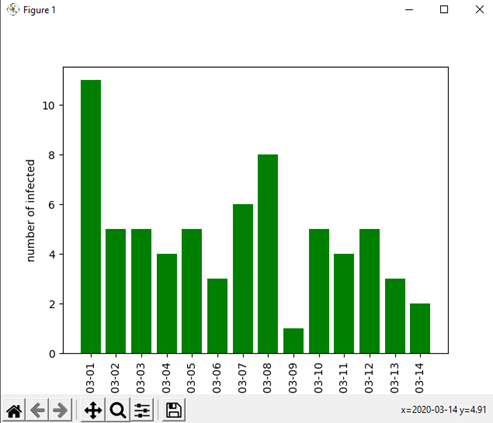
\includegraphics[scale=0.6]{./ex_query1.png}
             \caption{Example of the result of the above query plotted used the application described later}
        \end{figure}
		
		\subsection{Locations associated to infected people}
		\begin{code}
			\mycode{cypher}{query2.v}
		\end{code}
		The query aim is to find for each type of place, how many infected visited them in the last 2 days. The query is somehow pessimistic because it presume that all the infected people were already positive when they visited the Place.
		\subsection{People that went into contact with someone who got sick}
		The query’s goal is to find those people that met or visited the same place as someone who afterwards, in a set interval of time, turned out to be infected. According to our design this query divides into two subqueries:
		\begin{enumerate}
		    \item Here we want to check, for each infected individual, the places she visited the days prior the infection and match those people that visited that same place at the same date.
		    \begin{code} \mycode{cypher}{query3_1.v} \end{code}
		    
		   \item In this part we check for people that met and then one of them resulted positive.
		   \begin{code} \mycode{cypher}{query3_2.v} \end{code}
		\end{enumerate}
		The parameter “exposure\_interval” is how much back in time we search for potentially harmful contacts. The time granularity is of days and can be adjusted in the system files (by default is 5 days). The queries return the name and surname of the people potentially at risk of contagion, where and when the contact has occurred.
						  
						  
		\subsection{Find the average number of people met by infected ones, by kind of contact}
		\begin{code}
			\mycode{cypher}{query4.v}
		\end{code}
		This query exploits subqueries to find different values in only one execution. In our database we can find three kind of relationships that connect people, and this query aims is to find the average for each of them; to do so, we look for the total number of contacts between an infected individual and another person, but since there can be three different ways two people can connect, it is necessary to divide the query into three parts. In addition to that, there is one more subquery that finds the total number of infected people so that the avereages can be computed. In fact, if the averages were computed in the queries specific to each relationship, they would only show the average values according to the number of infected that fulfills at least one such relationship.\\
		Note that in this query only not infected people are considered while counting people met by infected ones, since the purpose of this query is to verify how the virus spreads to new, sane people.
				
		\subsection{Chart of number of people infected, subdivided by vaccine type (or no vaccine)}
		\begin{code}
			\mycode{cypher}{query5.v}
		\end{code}
		This query gets as result, for each vaccine type (or no vaccine) the number of people actually infected / positive tested. Notice that if a person has not been vaccinated, the attribute \texttt{p04\_vaccine} will be "no vaccine". After the execution of this query, a chart will be plotted to show how many people are infected for each vaccine type.
						  
		\subsection{Determine most effective vaccine}
		The most effective vaccine is calculated with a (simplified) formula:
		\begin{center}
			\texttt{\#of people infected with a certain vaccine / \# total amount of people vaccinated with the same certain vaccine}
		\end{center}
		In this case, we use 2 queries to get the result:
		\begin{itemize}
			\item The query at the previous point provides the number of people infected per vaccine
			\item Another query to retrieve the total number of people vaccinated per vaccine type:
		\end{itemize}
		\begin{code}
			\mycode{cypher}{query6.v}
		\end{code}
		Then, we simply calculate the ratio (via python code) using the results of the two queries and we take the absolute lowest ratio.
						  
		\section{Commands}
		\subsection{Add test}
		\begin{code}
			\mycode{cypher}{command1.v}
		\end{code}
		The aim of the above command is to add the result of a covid test executed in a certain date to the corresponding person. To perform this action the command uses the following parameters:
		\begin{itemize}
			\item \texttt{\$name}: the name of the patient;
			\item \texttt{\$surname}: the surname of the patient;
			\item \texttt{\$test\_type}: the type of the test to add to the patient;
			\item \texttt{\$date}: the date in which the test were executed;
			\item \texttt{\$test\_result}: the result of the test which is a boolean (true -> positive, false, negative).
		\end{itemize}
		Note that the command is designed in a way that allow the system to remain in a consistent state after the insertion of a new test record, and in particular two case are considered:
		\begin{itemize}
			\item if a person is tested positive, all the information about his infectivity state are update;
			\item if a positive person is tested negative, all the parameter about his infection period are resetted and this correspond in real life to the permission to end the quarantine period.  
		\end{itemize}
		\subsection{Add visit or meet relation}
		This command allows to add a contact occurred between two individuals, either because they were in the same monitored place in the same date or simply because they met at some point. Based on the previous cases the operations executed on the database are:
		\begin{code}\mycode{cypher}{command2_1.v}\end{code}
		and 
		\begin{code}\mycode{cypher}{command2_2.v}\end{code}
		It is also possible to add the event of a single person visiting a monitored place (by leaving the second and third row empty). If this is the case then we execute the following command:
		\begin{code}\mycode{cypher}{command2_3.v}\end{code}
		\subsection{Infect all families with at least 1 infected person}
		We know that the highest number of infections are related to family contacts, because it is easier to be infected when you use less cautions. So, we implemented a command to infect all families with at least 1 infected person, since this is a realistic scenario that appears quite frequently in real situations. The command is the following:
		\begin{code}
			\mycode{cypher}{command3.v}
		\end{code}
		
		Where \texttt{\$date} is a parameter that (conventionally) is setted at \texttt{"2020-03-15"}, that is the last date in our
		simulation.
		\subsection{Add vaccine dose}
		\begin{code}
			\mycode{cypher}{command4.v}
		\end{code}
		This simple command aims to add a single vaccine dose to a person's node. Two different scenarios are possible:
		\begin{itemize}
			\item if the objective is to add a dose of a certain vaccine to someone who has already had at least 1 dose of said vaccine, the number of doses will only increase by 1.
			\item if the objective is to add a dose of a certain vaccine to someone with no vaccine or with a different one, then the vaccine dose counter is increased by 1, while the vaccine type is overwritten as the latter is the most effective dose.
		\end{itemize}
				
		\subsection{Simulation}\label{sim}
		The creation of the dataset is entrusted to a function called simulatePandemic, it outputs a perfectly coherent dataset directly available for consultation in neo4j.\\
		On the first day (initial\_date in config.py file) it starts by infecting the initial number of people given by the user, after that it starts inspecting the relations that they had and by doing that it finds the individuals that are at risk of infection.\\
		Given a certain probability ( it depends on multiple editable factors stored in conf.py) a person who has been in contact with a sick individual can be infected by the virus.\\
		The set of ill people grows incrementally and so does the number of relations that need to be monitored by the application.
			\begin{code}
			\mycode{python}{command5.v}
		\end{code}
						  
						 
						  
						  
						  
		\section{Application}
		To make all the above queries and commands easy to use for the users, we developed an application with the related GUI.\\
		The application GUI is simply used to get the parameters necessary to run the query/command and to visualize the results of the queries.\\
		For a better understanding of the application, a copy of the whole project is available on the Github repository of the project and also a small demo is available on \href{https://youtu.be/C35U8NvhEVM}{YouTube link}.
						
		\pagebreak
						
		\pagebreak
		\clearpage
\end{document}